\section{Discussion}

Our results suggest that hash-based mesh remapping techniques offer a powerful alternative to traditional spatial data structures like kD-trees and quadtrees. The main advantages stem from their simpler control flow, better parallelism, and improved memory efficiency—particularly in heterogeneous environments like multi-core CPUs and GPUs.

In cases with structured or moderately unstructured AMR meshes, perfect hashes offer an efficient and collision-free remap solution. However, their memory footprint can become problematic in sparse mesh configurations. In these situations, compact hashing becomes advantageous by minimizing memory usage, though it introduces minor overhead due to sentinel value handling.

The hierarchical hash further provides a balanced solution for mixed-resolution meshes, especially where varying levels of refinement are present across the domain. This method effectively localizes memory operations and allows more control over spatial granularity.

Comparative tests with brute force methods (which scale as $\mathcal{O}(n^2)$) and tree-based methods (typically $\mathcal{O}(n \log n)$) confirm that hashing strategies consistently achieve better asymptotic and real-world performance. While brute force is often used for result validation due to its simplicity, it is not viable for large-scale simulations. Tree-based methods suffer from traversal overhead and are harder to optimize on parallel hardware due to recursive logic and synchronization issues.

It is worth noting that as meshes become increasingly unstructured or irregular—such as in real-time fluid dynamics or astrophysics simulations—the advantages of hashing become even more pronounced. The decoupling of data through hashing reduces the number of candidate intersections significantly and eliminates many expensive geometric calculations.

Future extensions of this work could explore dynamic hash-based remapping strategies and adaptive hash sizing to further optimize performance based on mesh characteristics and runtime conditions.

\begin{figure}[h]
  \centering
  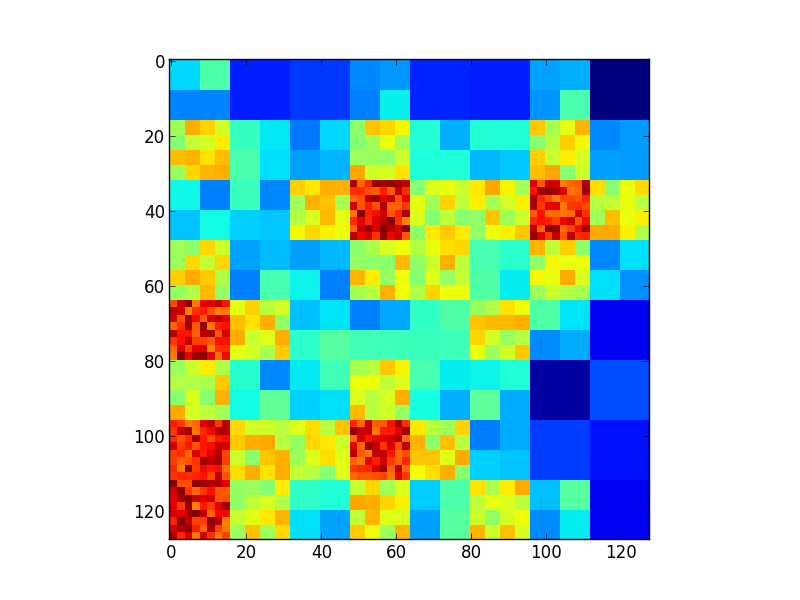
\includegraphics[width=0.75\textwidth]{./images/figure_p13_2.png}
  \caption{Summary visualization of method efficiency and suitability across mesh types.}
  \label{fig:discussion_summary}
\end{figure}

The idea of using attention mechanisms to reduce unnecessary computation draws inspiration from the transformer architecture~\cite{Vaswani2017}.
